\documentclass[11pt, oneside]{article}

\usepackage{harvard}
\setcounter{secnumdepth}{0} % don't number headings
\setcounter{page}{0} % title page 0

\usepackage{geometry}                % See geometry.pdf to learn the layout options. There are lots.
\geometry{letterpaper}                   % ... or a4paper or a5paper or ... 
\usepackage{fullpage}

%\geometry{landscape}                % Activate for for rotated page geometry
%\usepackage[parfill]{parskip}    % Activate to begin paragraphs with an empty line rather than an indent

\usepackage{graphicx}
\usepackage{amssymb}
\usepackage{epstopdf}
\DeclareGraphicsRule{.tif}{png}{.png}{`convert #1 `dirname #1`/`basename #1 .tif`.png}

\usepackage{array}
\newcolumntype{P}[1]{>{\centering\arraybackslash}p{#1}}
\newcolumntype{M}[1]{>{\raggedright\arraybackslash}m{#1}}

\newtheorem{hypothesis}{Hypothesis}

\usepackage{setspace}
\usepackage{multirow} 

\usepackage{graphicx}
\DeclareGraphicsExtensions{.pdf,.png,.jpg, .jpeg}
\usepackage{caption}
\usepackage{subcaption}
\usepackage{float}
\usepackage{afterpage}

\usepackage[margin=1in]{geometry}

\newcommand\T{\rule{0pt}{2.6ex}}       % Top strut
\newcommand\B{\rule[-1.2ex]{0pt}{0pt}} % Bottom strut

%%%%%%%%%%%%%%%%%%%%%%%%%
%%                       TITLE PAGE                       %% 
%%%%%%%%%%%%%%%%%%%%%%%%%

\title{Obsessed with Muslim Women's Rights? A Computational Text Analysis of U.S. News Coverage}
\author{Rochelle Terman\thanks{Corresponding author, \url{rterman@berkeley.edu}. } \\University of California, Berkeley\\Department of Political Science}
%\date{}                                           % Activate to display a given date or no date

\begin{document}
\maketitle
\baselineskip=2.00\baselineskip

\setcounter{page}{0}

\maketitle\thispagestyle{empty}

Replication Materials here: https://github.com/rochelleterman/worlds-women

\begin{center}
\textbf{PRELIMINARY DRAFT: PLEASE DO NOT CIRCULATE OR CITE WITHOUT PERMISSION}
\end{center}

\begin{abstract}
\noindent How does Congress exercise its constitutional role to advise on, and consent to, the nomination of federal judges? Much has been written about the confirmation process, both in the academic and popular literatures, but to date relatively little empirical research has focused on the content of the hearings themselves. Using semi-automated text analysis methods, we explore a new dataset of all nomination hearings held by the Senate Judiciary Committee between 2001-2012. In doing so, we begin to shed light on a largely unexplored ``black box'' of American politics: the substance and work-product of Congressional hearings.
\end{abstract}

\newpage\doublespace

\section{The Theory of Gendered Orientalism}

Since Edward Said's influential Orientalism, and especially after 9/11, a large literature has developed critiquing American media coverage of women in Muslim, Arab, and Middle Eastern societies. While the literature spans multiple disciplines, theoretical approaches, and empirical territory, scholars converge on three modal claims. First, American media discourse is purportedly``obsessed" with Muslim women's oppression. Popular media outlets portray Middle Eastern, Arab, and Muslim societies as uniquely or particularly misogynistic, especially compared to Western countries. This misogyny is ascribed to Islam and/or Arab culture, which is said to justify or require female subjugation. Not only is this narrative simplistic and sensationalist, it conflicts with the reality of women's lives insofar as it inaccurately portrays the degree and cause of Muslim women's suffering. Furthermore, it denies women's agency by reduces their lives to a totalizing oppression , while demonizing Muslim, Arab, and Middle Eastern men as inherently barbaric and cruel. 

Second, American media discourse tend to compare the lives of Muslim women to those of Western women, who are portrayed, by contrast, as liberated and free by comparison. Together, this dichotomy justifies a rescue mission by which Western feminists must ``save'' Muslim women from their oppressive religion (i.e. Islam), culture, or traditions. The ``savior'' narrative has been heavily scrutinized by feminist and critical scholars, who denounce it as paternalistic and imperialist. 

Third, the need to ``save'' Muslim women, bolstered by American media portrayals, is often used to justify undesirable political imperatives, including military intervention, repressive or exploitative policies, and cultural imperialism. In many cases, the plight of women is not the central concern; rather, it is used cynically as a way to bolster public support for international aggression. The increased coverage of Afghan women post 9/11 is an oft-cited case in point, but scholars have also looked to historical cases in which footbinding (Teng1996), female genital mutilation (?), sati, and polygamy were used to legitimize colonialism. In other words, American media coverage of Muslim women is largely determined by political imperatives, and the distribution of attention on women's issues mirrors the contours of American geopolitical interests and foreign policy.

Together, these three claims make up a general argument that I call ``gendered orientalism,'' and provide the foundation for a sprawling literature and even a number of subfields. But while rising to the level of common sense in some disciplines, the argument is treated with suspicion in others, perhaps due to the literature's general prioritization of theoretical innovation over empirical findings. This is not to say that empirical evidence is entirely absent. Indeed, qualitative research on the topic has generated a number of insightful case studies, especially on the post 9-11 Afghan case, while a few medium-N content analyses have explored the phenomenon in greater scope. These works not withstanding, we have yet to see a quantitative analysis that is able to test these claims against a large empirical dataset. 

Such a study is difficult due to the practical challenges involved in creating a large-scale, systematic, and comparative analysis of U.S. media coverage of Muslim and Middle Eastern women. Fortunately, newly available data sources and methodological tools in the realm of computational text analysis have opened the door to novel empirical possibilities. By virtue of their methodological limitations, such techniques could never replace careful qualitative work or rich theoretical analyses. But they would provide another lens through which we could evaluate an argument that has become so essential to such a large body of work.

\subsection{Hypotheses}

When scholars of gendered orientalism say that the U.S. media are obsessed with Muslim women's oppression, it is not immediately clear what they mean. What possible mechanisms can we infer from the theory that we can then test empirically? One possible mechanism involves the relationship between stereotype and confirmation bias. Few scholars would deny the existence of sexism or women's oppression in Middle Eastern or Muslim societies. But they would argue that women's oppression in Muslim countries tend to be noticed more often than women's oppression in Western countries, which are elided under the latent assumption of gender equality in these societies. In this way, American media are influenced by the stereotype that Muslim and Middle Eastern countries are uniquely or especially sexist, and perpetuate that stereotype via confirmation bias. 

This leads to a testable hypothesis: women's oppression in Muslim societies is considered more news-worthy, while women's oppression in Western societies is ignored. In other words, we would predict an inverse relationship between women's status and the quantity of news coverage about women in Muslim versus non-Muslim countries. Among Middle Eastern and Muslim-majority countries, American news media will tend to report more stories about women the greater inequality they face. But in other countries, women are more likely to be represented when they have relatively high political, social, and economic status. 

\begin{hypothesis}
Women's status is negatively correlated with the quantity of U.S. news coverage of Muslim and Middle Eastern countries, but positively correlated in other cases.
\end{hypothesis}

While the first proposed mechanism has to do with quantity of coverage, a second possible mechanism centers around the tone or framing of such coverage. Not only is Muslim women's oppression reported on more often in the American press; their entire lives are reduced to this supposed oppression or inequality. Western women, on the other hand, are reported in higher dimensions and with more complexity, according to the gendered orientalism argument.

This, too, generates a testable hypothesis. News coverage of women can take on a variety of content, from rights and equality to sports, fashion, travel, etc. If we believe the gender orientalist argument, however, we would expect coverage of Muslim or Middle Eastern women to feature a more concentrated discussion of women's rights and gender (in)equality compared to coverage of women in non-Muslim or European countries. We would also expect the proportion of coverage dedicated to women's rights to be higher regardless of women's actual status in these countries. In other words, if we take a Muslim country and a non-Muslim country with equivalent records of women's rights, we would expect that American news media will focus more on gender equality in the Muslim case compared to the non-Muslim case.

\begin{hypothesis}
U.S. news coverage of women in Muslim and Middle Eastern countries will focus more on women's rights and gender equality, relative to other topics, compared to non-Muslim and non-Middle Eastern countries, even when controlling for women's political, social, and economic status.
\end{hypothesis}

\subsection{Data}

The primary data used in this study consists of all articles about women in non-U.S. countries, published in the \emph{New York Times} and \emph{Washington Post}, 1980--2014. Clearly, the inferences drawn from this data cannot be straightforwardly applied to American media writ large. With that reservation, however, there are still reasons to value this sample. In addition to being available to researchers, these two outlets are often considered ``papers of record," i.e. the most prominent, accurate, and influential among U.S. news media. These sources are especially prominent among the foreign policy establishment due to their reputation for reporting of international affairs. Other media outlets, including print and television news, rely on the New York Times and Washington Post for their reporting (Schraeder and Endless 1998).  Finally, the 35-year sample includes enough variation in geopolitical affairs to validly test the hypotheses raised above.

Using the LexisNexis database, I downloaded all articles containing the subject term ``women" from these two outlets during the specified time period. Subject terms are derived from LexisNexis's SmartIndexing technology, which applies controlled vocabulary terms for different taxonomies such as subject, geographic region, language, etc. In addition to subject, documents are assigned country terms along with a relevance score that calculates how important or salient each country is to a document. Scores of 85 percent or higher indicate a major term. I assign each article to a single country using its most salient country term, if that term has a relevance score of 85 percent or higher. Articles with missing major country terms were discarded.\footnote{\hspace{5}Some articles contained more than one major country term; in these cases, I took the term with the highest relevance score. These cases accounted for only 9 per cent of the corpus.}  Because this study explores how U.S. media represent women abroad, I discarded all articles that were primarily about the United States. The final sample includes 4522 documents: 3720 from the New York Times and 802 from the Washington Post. 

These data were then combined into a country-year data set, with each document assigned to an observation based on the year in which it was published and the country it most concerned. The country-year data set includes all current and historic U.N. states, plus Palestine but excluding the United States, for a total of 198 countries and 6226 observations. 

County-years were assigned a regional classification loosely based on Hafner-Burton and Ron's (2012) six regional groupings: \emph{Powerful West} (West) with 28 countries; \emph{Asia} (Asia) with 33 countries, including Pakistan; \emph{Latin America} (LA) with 33 countries; the \emph{Middle East and North Africa} (MENA) with 22 countries, including Afghanistan; \emph{Sub-Saharan Africa} (Africa), with 46 countries; and the \emph{Eastern Europe and Central Asia} (EECA) with 31 countries. These regional groupings generally conform to the United Nations' regional classification, with some exceptions. First, former countries are assigned to regions based on where their current territorial manifestations are classified. Second, due to ambiguity surrounding whether Pakistan and Afghanistan are part of the Middle East or Asia, I decided to code these countries based on their assignment in most U.S. higher education area studies programs, with Afghanistan going in MENA and Pakistan in Asia; these assignments generally reflect the location of these nations in U.S. popular consciousness. Finally, the Powerful West is a region that Hafner-Burton and Ron include in their study and that I agree is important given the theoretical argument we wish to test. This region includes advanced industrialized countries of North American and Western Europe, along with two highly developed Asian countries -- Australia and New Zealand.

\begin{figure}[h]
\caption{Number of Articles per Region over Time}\label{fig:n-region}
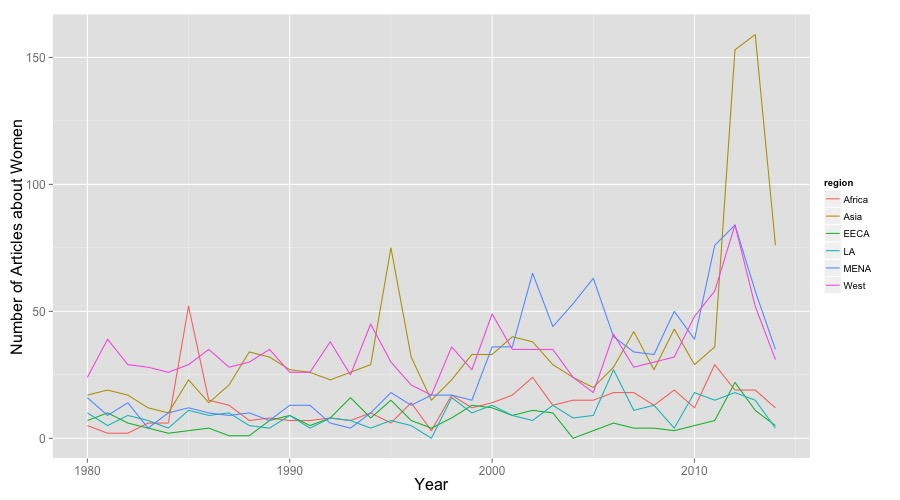
\includegraphics[scale=0.55]{n-region-plot}
\end{figure}


\section{Modeling Hypothesis 1}

The first hypotheses pertains to the likelihood of U.S. news coverage on women. Here, the dependent variable (likelihood of U.S. news coverage of women) is operationalized in two ways. The first is a simple binary (\emph{Reported}) indicating whether a country-year observation was covered in the documents (true in 1451 cases). Second, I recorded the total number of articles about women for that observation (\emph{Document Count}). 

Hypothesis 1 claims that the effect of women's rights on the likelihood of coverage is conditional on whether the unit of observation is a Muslim or Middle East country. Thus an interaction term is necessary for the model. \footnote{Clearly, respect for women's rights is itself affected by whether the observation is a Muslim or MENA country. However, tests using variable inflation factors indicate that collinearity was not a problem in the models, and, furthermore, the results are robust across a number of specifications.} The mediating variable (Muslim or Middle Eastern country) is operationalized in three ways: \emph{Percentage Muslim} captures the Muslim percentage of a population according to research by the Pew Research Center. \emph{Muslim Majority} is a binary indicating whether the \emph{Percentage Muslim} is 50 per cent or above. \emph{MENA} is a binary indicating whether a country is included in the Middle East and North Africa regional classification described above. I estimate models with all three measures in order to compare potential causal mechanisms. 

Modeling \emph{Women's Rights}, or the material condition of women's rights and gender equality, is problematic due to the conceptual difficulties surrounding this term (Peksen 2011). While recognizing the limitations of such a measure, I rely on the popular Cingranelli-Richards Rights Index (CIRI), which culls data from the U.S. State Department's annual human rights country reports. This is appropriate for the task at hand, because we would expect that U.S. news media follow a commensurate understanding of ``women's rights'' with that used by the U.S. State Department. CIRI offers three variables capturing the notion of women's rights as they are effected in law and practice: \emph{Women's Economic Rights}, \emph{Women's Political Rights}, and \emph{Women's Social Rights}.\footnote{\hspace{5}The \emph{Women's Political Rights} variable include the following rights: ``The right to vote; the right to run for political office; the right to hold elected and appointed government positions; the right to join political parties; the right to petition government officials." \emph{Women's Social Rights} includes: ``The right to equal inheritance; the right to enter into marriage on a basis of equality with men; the right to travel abroad; the right to obtain a passport; the right to confer citizenship to children or a husband; the right to initiate a divorce; the right to own, acquire, manage, and retain property brought into marriage; the right to participate in social, cultural, and community activities; the right to an education; the freedom to choose a residence/domicile; freedom from female genital mutilation of children and adults without their consent; freedom from forced sterilization. \emph{Women's Economic Rights} is coded based on the following: ``Equal pay for equal work; free choice of profession or employment without the need to obtain a husband or male relative's consent; the right to gainful employment without the need to obtain a husband or male relative's consent; equality in hiring and promotion practices; job security (maternity leave, unemployment benefits, no arbitrary firing or layoffs, etc.); non-discrimination by employers; the right to be free from sexual harassment in the workplace; the right to work at night; the right to work in occupations classified as dangerous; the right to work in the military and police force."  (Cingranelli and Richards 2012)}  Each variable is an ordinal variable ranging from 0 (indicating that women's rights were not guaranteed by law during a given year) to 3 (indicating that women's rights were guaranteed in both law and practice.)\footnote{\hspace{5}The \emph{Women's Political Rights} and \emph{Women's Economic Rights} variables are only available to 2011. The \emph{Women's Social Rights} variable is only available to 2004.} The composite variable \emph{Women's Rights} estimates the overall situation of women's rights by taking the mean of these three indicators.\footnote{\hspace{3} The results are robust when using the three individual indices in place of the composite variable. See Appendix}  

I include a number of controls that may affect the likelihood of coverage. First, a straightforward alternative explanation suggests that reporting about women is proportional to general news coverage. The variable \emph{Country Reports} records the number of articles that appear in the \emph{New York Times} relating to a particular country-year, including those that are unrelated to the subject ``women." We would expect coverage about women to be highly correlated with general coverage for a given country-year.

On the other hand, articles about women may exhibit special features that make it different from general reporting. For instance, journalists may treat stories about women as ``softer'' news, requiring more personal interviews and field research than ``hard'' news items. One implication is that journalists may find it difficult to report on authoritarian countries, which tend to restrict freedoms of speech, assembly, and the press. To account for this possibility, I include a \emph{Democracy} variable from the Polity IV dataset's Polity2 index, which is constructed by subtracting the 10-point autocracy index that measures the autocratic features from the 10-point democracy index that identifies the democratic characteristics of a polity (Marshall and Jaggers 2002).\footnote{\hspace{5}This data is only available to 2013.} Therefore, \emph{Democracy} ranges from --10 (most autocratic) to +10 (most democratic). 

Similarly, journalists may find it difficult to report on countries that are mired in domestic turmoil and violence. Thus I include a variable \emph{Instability} culled from the Banks Cross-National Time Series Data Archive composite index of political instability, which encompasses multiple indicators including riots, antigovernment protests, guerrilla attacks, general strikes, purges, government crises, and assassinations. Higher values on this scale denote greater levels of political unrest and violence. 

Finally, I include controls for \emph{GDP per capita} (logged) using World Bank Development Indicators and \emph{Population} (logged) using data from the United Nations. The rationale is that journalists find it easier to report about women in rich, populous countries, where it is easier to conduct field research and/or conduct interviews. 

I use statistical models that account for the cross-national time-series structure of the data. Because the panel data are highly correlated, I use generalized estimating equations (Zorn 2001). When modeling the dependent variable using the \emph{Reporting} binary, I use a probit regression. When modeling the dependent variable using \emph{Document Counts}, I use a negative binomial regression since this variable consists of over-dispersed counts. Note that a tobit is inappropriate here because coverage cannot assume negative values. PAPER. To deal with heteroskedasticity, all estimates use Huber-White corrected robust standard errors clustered on country.  Time-variant independent and control variables are lagged by one year to mitigate simultaneity issues and lessen any incorrect direction of inference. I also include a lagged-dependent variable in some models to correct for serial correlation (Wooldridge 2002). The results are summarized in Tables \ref{table:logit} and \ref{table:negbin}.


% Table created by stargazer v.5.1 by Marek Hlavac, Harvard University. E-mail: hlavac at fas.harvard.edu
% Date and time: Thu, Sep 24, 2015 - 17:25:44
\begin{table}[!htbp] \centering 
  \caption{Testing Hypothesis 1 with \emph{Reported} (Binary) DV}
  \label{table:logit} 
\begin{tabular}{@{\extracolsep{5pt}}lccc} 
\\[-1.8ex]\hline \\[-1.8ex] 
%\\[-1.8ex] & \multicolumn{3}{c}{\textbf{Reported (Binary)}} \\ 
\\[-1.8ex] & \textbf{Model 1} & \textbf{Model 2} & \textbf{Model 3}\\ 
\hline \\[-1.8ex] 
 Lagged DV & 0.494$^{***}$ & 0.495$^{***}$ & 0.495$^{***}$ \\ 
  & (0.061) & (0.061) & (0.061) \\ 
  Country Reports & 0.002$^{***}$ & 0.002$^{***}$ & 0.002$^{***}$ \\ 
  & (0.0003) & (0.0003) & (0.0003) \\ 
  Women's Rights Index & 0.080 & 0.087 & 0.102 \\ 
  & (0.066) & (0.064) & (0.069) \\ 
  Muslim Majority & 0.438$^{***}$ &  &  \\ 
  & (0.166) &  &  \\ 
  MENA &  & 0.552$^{***}$ &  \\ 
  &  & (0.183) &  \\ 
  Muslim Percentage &  &  & 0.512$^{***}$ \\ 
  &  &  & (0.185) \\ 
  Democracy & 0.007 & 0.011$^{**}$ & 0.007 \\ 
  & (0.005) & (0.005) & (0.005) \\ 
  Instability & $-$0.00001 & $-$0.00001 & $-$0.00001 \\ 
  & (0.00002) & (0.00002) & (0.00002) \\ 
  Population & 0.381$^{***}$ & 0.379$^{***}$ & 0.376$^{***}$ \\ 
  & (0.023) & (0.023) & (0.023) \\ 
  GDP per capita & 0.133$^{***}$ & 0.119$^{***}$ & 0.131$^{***}$ \\ 
  & (0.024) & (0.025) & (0.024) \\ 
  Women's Rights x Muslim Majority & $-$0.372$^{***}$ &  &  \\ 
  & (0.127) &  &  \\ 
  Women's Rights x MENA &  & $-$0.342$^{**}$ &  \\ 
  &  & (0.142) &  \\ 
  Women's Rights x Muslim Percentage &  &  & $-$0.392$^{***}$ \\ 
  &  &  & (0.138) \\ 
  Constant & $-$8.310$^{***}$ & $-$8.212$^{***}$ & $-$8.265$^{***}$ \\ 
  & (0.443) & (0.442) & (0.441) \\ 
 N & 3962 & 3962 & 3946 \\ 
Log Likelihood & $-$1653.813 & $-$1653.581 & $-$1648.084 \\ 
AIC & 3327.627 & 3327.162 & 3316.168 \\ 
\hline \\[-1.8ex] 
\multicolumn{4}{l}{$^{***}$p $<$ .01; $^{**}$p $<$ .05; $^{*}$p $<$ .1} \\ 
\multicolumn{4}{l}{Robust standard errors clustered on country appear in parentheses.} \\ 
\end{tabular} 
\end{table} 


% Table created by stargazer v.5.1 by Marek Hlavac, Harvard University. E-mail: hlavac at fas.harvard.edu
% Date and time: Thu, Sep 24, 2015 - 17:20:04
\begin{table}[!htbp] \centering 
  \caption{Testing Hypothesis 1 with \emph{Document Count} DV}
    \label{table:negbin} 
\begin{tabular}{@{\extracolsep{5pt}}lccc} 
\\[-1.8ex]\hline \\[-1.8ex] 
%\\[-1.8ex] & \multicolumn{3}{c}{\textbf{Document Count}} \\ 
\\[-1.8ex] & \textbf{Model 1} & \textbf{Model 2} & \textbf{Model 3}\\ 
\hline \\[-1.8ex] 
 Lagged DV & 0.147$^{***}$ & 0.149$^{***}$ & 0.149$^{***}$ \\ 
  & (0.013) & (0.013) & (0.013) \\ 
  Country Reports & 0.001$^{***}$ & 0.001$^{***}$ & 0.001$^{***}$ \\ 
  & (0.0002) & (0.0001) & (0.0002) \\ 
  Women's Rights Index & 0.118 & 0.154$^{*}$ & 0.153 \\ 
  & (0.096) & (0.093) & (0.103) \\ 
  Muslim Majority & 1.058$^{***}$ &  &  \\ 
  & (0.319) &  &  \\ 
  MENA &  & 1.298$^{***}$ &  \\ 
  &  & (0.340) &  \\ 
  Muslim Percentage &  &  & 1.166$^{***}$ \\ 
  &  &  & (0.352) \\ 
  Democracy & 0.006 & 0.018$^{*}$ & 0.007 \\ 
  & (0.010) & (0.010) & (0.010) \\ 
  Instability & $-$0.00001 & $-$0.00001 & $-$0.00000 \\ 
  & (0.00002) & (0.00002) & (0.00002) \\ 
  Population & 0.528$^{***}$ & 0.539$^{***}$ & 0.521$^{***}$ \\ 
  & (0.026) & (0.027) & (0.026) \\ 
  GDP per capita & 0.209$^{***}$ & 0.169$^{***}$ & 0.209$^{***}$ \\ 
  & (0.036) & (0.037) & (0.036) \\ 
  Women's Rights x Muslim Majority & $-$0.821$^{***}$ &  &  \\ 
  & (0.205) &  &  \\ 
  Women's Rights x MENA &  & $-$0.581$^{***}$ &  \\ 
  &  & (0.215) &  \\ 
  Women's Rights x Muslim Percentage &  &  & $-$0.825$^{***}$ \\ 
  &  &  & (0.218) \\ 
  Constant & $-$11.635$^{***}$ & $-$11.641$^{***}$ & $-$11.579$^{***}$ \\ 
  & (0.623) & (0.632) & (0.629) \\ 
 N & 3962 & 3962 & 3946 \\ 
Log Likelihood & $-$3576.578 & $-$3566.883 & $-$3569.499 \\ 
$\theta$ & 0.905$^{***}$  (0.061) & 0.933$^{***}$  (0.064) & 0.907$^{***}$  (0.061) \\ 
AIC & 7173.156 & 7153.767 & 7158.999 \\ 
\hline \\[-1.8ex] 
\multicolumn{4}{l}{$^{***}$p $<$ .01; $^{**}$p $<$ .05; $^{*}$p $<$ .1} \\ 
\multicolumn{4}{l}{Robust standard errors clustered on country appear in parentheses.} \\ 
\end{tabular} 
\end{table} 

The models provide strong support for Hypothesis 1. 

\begin{figure}
\begin{subfigure}{.5\textwidth}
  \centering
  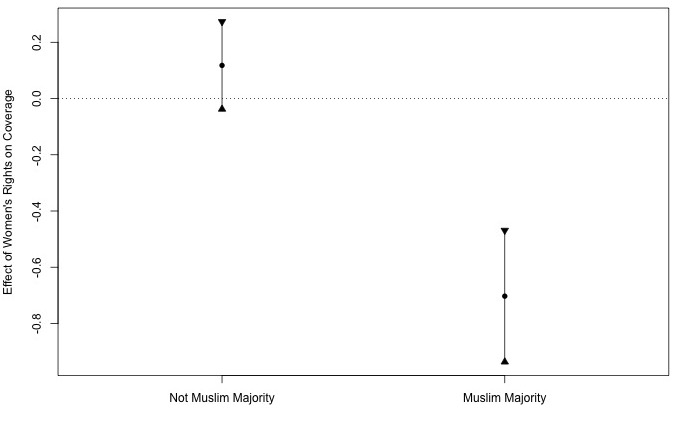
\includegraphics[width=1\linewidth]{nb1}
  \caption{Interaction with \emph{Muslim Majority}}
  \label{fig:sfig1}
\end{subfigure} 
\begin{subfigure}{.5\textwidth}
  \centering
  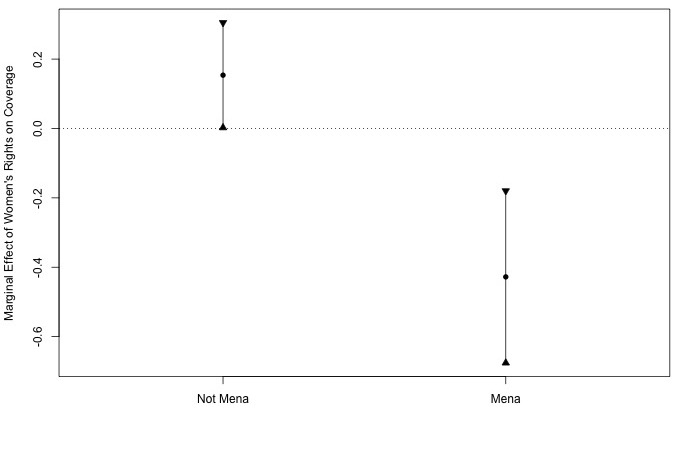
\includegraphics[width=1\linewidth]{nb2}
    \caption{Interaction with \emph{MENA}}
  \label{fig:sfig2}
\end{subfigure}
\begin{subfigure}{.5\textwidth}
\vspace{.5cm}
  \centering
  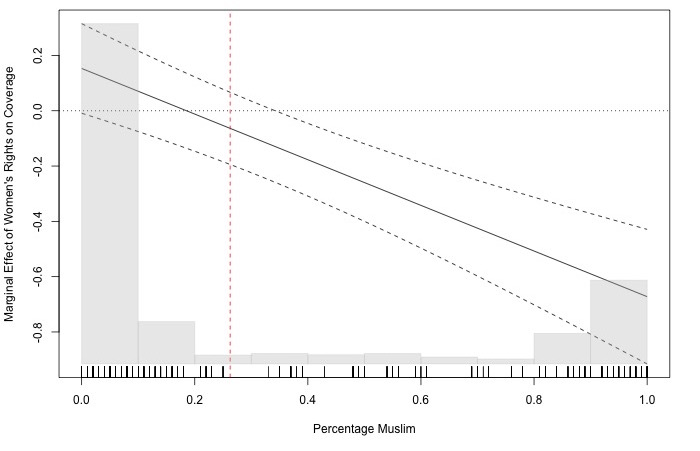
\includegraphics[width=1\linewidth]{nb3}
    \caption{Interaction with \emph{Muslim Percentage}}
  \label{fig:sfig2}
\end{subfigure}
\vspace{.5cm}
\caption{Marginal Effect of \emph{Women's Rights} on \emph{Document Count}}
\label{fig:fig}
\end{figure}

The findings are robust across a number of specifications. First, I ran alternative models replacing the \emph{Women's Rights Index} composite variable with individual scores representing \emph{Women's Political Rights}, \emph{Women's Social Rights}, and \emph{Women's Economic Rights} respectively. Second, to address potential bias stemming from missing data on covariates, I model effects using two imputation methods: a "nearest value" method, whereby I impute covariate data using the last reported value at the country level; and a multiple imputation method as as described by King et al (2001.\footnote{\hspace{5}I use the \emph{Amelia} package in $R$ to estimate missing data using multiple imputation. Honaker et al. 2011)} Finally, I estimated models without the lagged dependent variable, and removing Israel from the sample if MENA countries. The results with substantively equivalent across all models.\footnote{\hspace{5}All models are included in the Appendix.}

\section{Measuring Topical Focus in Women's Rights Coverage}

The second hypotheses pertains to the quality of coverage about women abroad, suggesting that U.S. news coverage of women in Muslim and Middle Eastern countries will focus more on women's rights and gender equality, relative to other topics. This requires us to estimate the distribution of topics in the corpus of articles. Fortunately, recent advances in computational tools for the analysis of textual data enable new tools used to categorize, summarize, scale, and compare texts (J. Grimmer and Stewart 2013). Among the most promising tools for social scientists and humanists, and the chief method used in this paper, is the probabilistic topic model, an algorithm used to code the content of a corpus of texts into substantively meaningful categories, or ``topics," using the statistical correlations between words in a corpus (Mohr and Bogdanov 2013).

As a demonstration, imagine we have two sets of documents, one about food and the other about sports. We would expect that, given a document is about a particular topic, certain words would appear more or less frequently. ``Sports" and ``athlete" would appear more often in documents about sports, while ``food" and ``ingredient" would appear in documents about food, and ``is" would appear equally in both. A topic model captures this intuition in a statistical framework, discovering abstract topics that might be thought of as a constellation of words that tend to come up in conversation (Mohr and Bogdanov 2013). 

The benefits of this method lie in its ability to infer and analyze substantively meaningful categories (topics) with minimal assumptions and expense (Quinn et al. 2010). Unlike human-coder approaches, an automated topic model estimates topics from the observed data without assuming the substance, division, or keywords of topics beforehand. Thus it ameliorates the potential for confirmation bias (Nelson 2015, 21). It is also fully replicable, because it is fully automated, which is an important validity concern for content analysis (Neuendorf 2011). 

To identify and explore the thematic topics in U.S. news media reporting about women abroad, I use the Structural Topic Model, developed by Roberts et al (2013) with the goal to ``help researchers understand relationships between metadata and topics in their text corpus" (Lucas et al. 2015, 2). The Structural Topic Model (STM) extends the popular topic modeling tool called Latent Dirichlet Allocation (LDA) by incorporating document-level metadata into the analysis as covariates. This allows us to measure systematic changes in topical prevalence according to changes in metadata, similar to a regression framework (Roberts et al. 2014, 5). 

\subsection{Data Preparation}

To estimate the topic model, the corpus was first preprocessed following the standard recipe for automated text analysis. First, I removed capitalization, numbers, and punctuation. I then removed stop words, or those words that are extremely common but unrelated to the research topic, such as ``and,'' ``or,'' ``the," etc.  I then applied a stemming algorithm to the corpus, which reduces words to their stem or root, using the Porter Snowball II stemmer for English, widely used in many automated text analysis applications (Porter 2001). I also removed sparse terms by discarding all words used in only one or two documents out of the entire corpus. 

In a less common step, I removed named entities such as the names of specific people, locations, and organizations, from the text of the articles. The reasoning behind this decision is that including terms that are specific to a particular region -- such as the names of countries or political leaders -- would potentially bias the model to infer topics that are essentially regional categories instead of thematic ones. Because I am interested in the relationship between substantive topics and region, I chose to remove such terms, which I identified using Stanford's Named Entity Recognizer as well as my own dictionary of nationalities.

Once pre-processing was completed, the remaining words were transformed into a vector containing the count of each unique word in a document, disregarding information such as the order in which the words appear.  The vectors are combined to construct a document-term matrix (DTM), where each row represents a document, each column represents a unique word, and each cell is the count of a unique word in a particular document. The final corpus had 4522 documents, 15,300 unique words and 1,047,653 total words. This DTM is the primary input for the structural topic model. 
	
\subsection{Model Selection and Topics}

When estimating an STM, the analyst must make a number of important decisions pertaining to model selection. First, she must specify the number of topics ($K$) to be estimated. There is no one answer for this decision (Roberts et al. 2014). The choice of $K$ depends on a number of factors, including the nature of the documents under study and the level of granularity the analyst wishes to capture. In addition, STM depends on a multi-modal objective function, meaning that models with the same parameters (that is, the same data, covariates, and number of topic) may produce different results -- that is, different topics -- depending on the starting seed value.

Generally speaking, the best topic model is the one that generates the highest quality topics, and a higher quality topic is one that displays a higher degree of semantic interpretability. Two measures exist to evaluate interpretability quantitatively: cohesiveness and exclusivity. A topic is cohesive if its top words are likely to co-occur within documents. It is exclusive if top words are unique to that topic, or unlikely to appear in the top words for another topic (Roberts et al. 2014, 6). Oftentimes scholars will generate a number of candidate models and then discard those with low degrees of exclusivity and cohesiveness given a set $K$ (Roberts et al. 2014).

Even with these tools, however, selecting a model usually requires human judgment to evaluate the semantic meaning of topics (Mohr and Bogdanov 2013). For instance, we can try to summarize a topic by seeing which words have the highest probability of appearing in a topic. But because LDA topics are a distribution over all words, this technique usually prioritizes words that have high frequency in the entire corpus, but may not be semantically informative (i.e. ``women" in this case). Another technique is to identify words that are exclusive to that topic, such as simplified frequency-exclusivity scoring (FREX) (Lucas et al. 2015, 5). A third technique is to see which document is most representative of a topic and read it to infer the topic's content.

To address model specification issues, I estimated over 50 models varying the number of topics and starting seed values, and relied on the techniques described above to choose the highest quality model and apply semantic labels to each topic in that model. I did not look at corpus or region-level topic distributions before choosing a model to prevent bias. The final model estimated 15 topics by regressing topic prevalence on region and year covariates. Table \ref{table:labels} gives a summary of those topics, including each topic's semantic label (applied by me), as well as top words calculated by frequency and FREX metrics.\foonote{The words reported are stemmed, as explained above.} There is a clearly discernible topic corresponding to ``Women's Rights \& Gender Equality" in this corpus, as inferred by the words \emph{right, equal, discrimin}, etc. Figure X gives the topics' exclusivity and cohesiveness scores.

\afterpage{\clearpage}
% latex table generated in R 3.2.1 by xtable 1.7-4 package
% Mon Sep 21 15:04:36 2015
\begin{table}[!p]
\centering
\small
\caption{Summary of Topic Labels}\label{table:labels}
\begin{tabular}{p{.3cm} M{4cm} | M{5cm} | M{5 cm} }
  \hline \hspace{5}
 & Labels & Probability & FREX \T\B \\ 
  \hline \\
1 & Cancer & women, said, cancer, studi, breast, research, drug & cancer, implant, hormon, tumor, virus, breast, pill \\  &&&\\
  2 & Reproductive Health & abort, health, women, countri, children, birth, year & abort, birth, health, matern, aid, childbirth, pregnant \\ &&&\\
  3 & Religion & said, islam, religi, women, church, countri, ian & islam, religi, secular, circumcis, fundamentalist, koran, religion \\ &&&\\
  4 & Business \& Work & women, said, percent, work, compani, year, job & ese, compani, corpor, board, employ, bank, job \\ &&&\\
  5 & Marriage \& Family & said, famili, husband, girl, mother, year, children & father, husband, daughter, son, villag, bride, sister \\ &&&\\
  6 & Arts & art, work, show, artist, page, perform, photograph & museum, sculptur, artist, painter, art, galleri, exhibit \\ &&&\\
  7 & Migration & said, worker, citi, work, year, prostitut, govern & factori, brothel, prostitut, traffick, tourist, worker, migrant \\ &&&\\
  8 & Gender-Based Violence & said, rape, polic, case, report, sexual, violenc & rape, crime, prosecutor, crimin, prosecut, sentenc, victim \\ &&&\\
  9 & War \& Combat & said, women, war, militari, kill, attack, soldier & soldier, troop, militari, combat, bomb, command, gun \\ &&&\\
  10 & Literature & book, film, write, stori, life, woman, love & novel, reader, film, charact, write, edit, literari \\ &&&\\
  11 & Human Interest & like, say, one, women, can, just, peopl & think, see, thing, feel, someth, realli, just \\ &&&\\
  12 & Women's Rights \& Gender Equality & women, right, law, men, said, issu, equal & law, equal, discrimin, constitut, legal, bill, divorc \\ &&&\\
  13 & Politics & said, polit, presid, govern, minist, elect, parti & elect, deleg, vote, voter, confer, minist, prime \\ &&&\\
  14 & Sports & team, women, game, said, world, play, olymp & game, olymp, sport, player, soccer, coach, athlet \\ &&&\\
  15 & Fashion & women, dress, fashion, wear, design, cloth, said & jacket, coutur, kimono, fashion, shirt, silk, skirt \\ &&&\\
   \hline
\end{tabular}
\end{table}

\footnote{\hspace{5} Applying semantic labels is more of an art than a science, because topics are merely statistical distributions of words, not hermeneutic concepts. Thus the ``Politics" topic should not be considered all-encompassing of every aspect of political life; rather, it is a heuristic shortcut for a constellation of words that relate to specifically electoral politics (e.g. \emph{polit, presid, govern, elect, minist, parti}.} \footnote{\hspace{5} Some topics are more easily interpretable than others. The ``Sports" topic, for instance, is fairly straightforward. The ``Human Interest" topic, on the other hand, requires more thought because its top frequency words are ubiquitous and vague (s\emph{aid, say, like, one, just, peopl, women}). More enlightening are the ``Human Interest" topic's top FREX words (\emph{think, feel, know, thing, realli, see, someth}), which suggest individual perspectives over facts and events. Reading the most representative documents, i.e. those with the highest percentage of its content devoted to the topic, offers the most insight. The most representative documents are interviews, profiles, inspiring stories of remarkable individuals, and so on. Taken together, I applied the label ``Human Interest" because the topic appears to capture human interest reporting.}

\subsection{Comparing Coverage across Region}

As a reminder, each document is represented as a mixture of these topics. For example, a hypothetical document devotes 54 percent of its content to ``Business \& Work," 14 percent of its content to ``Women's Rights \& Gender Equality," 7 percent of its content to ``Marriage \& Family," etc. Knowing this, we can calculate a number of summary statistics for topic distributions across the corpus. Figure \ref{fig:summary} gives a corpus-level summary of topic distributions. The most common topics are ``Women's Rights \& Gender Equality," ``Human Interest," and ``Politics," with the average document devoting about 10-12 percent of its content to each of these topics. ``Arts" is the least common topic, accounting for about 4 percent of the corpus' content.

\begin{figure}[h]
\begin{center}
\caption{Corpus Summary}\label{fig:summary}
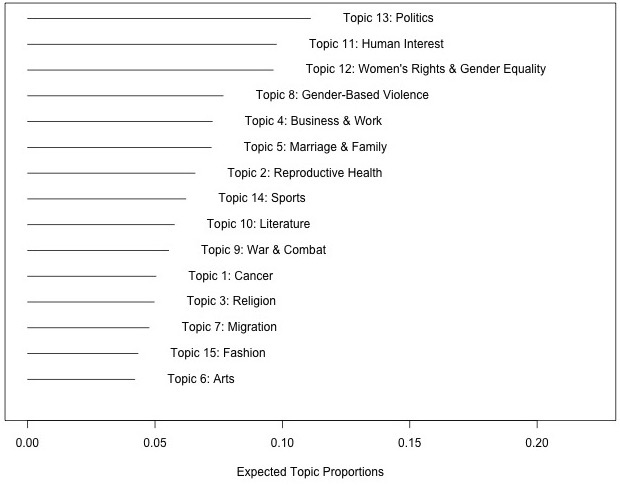
\includegraphics[scale=0.65]{corpus}
\end{center}
\end{figure}

Coverage of these topics is unevenly distributed across regions. Table \ref{table:region-distr} tabulates the proportion of each topic (using the number of words assigned to it in the model) devoted to each region. As we can see, almost a third of American news coverage about ``Women's Rights \& Gender Equality'' abroad is dedicated to countries in the Middle East. These statistics, it should be noted, are not normalized for the total number of articles coming from each region. But even when we account for the population of articles, we see that regions vary greatly in their average content. 

% latex table generated in R 3.2.1 by xtable 1.7-4 package
% Mon Sep 21 21:03:52 2015
\begin{table}[ht]
\centering
\caption{Topical Coverage across Region}\label{table:region-distr}
\begin{tabular}{lrrrrrrr}
  \hline
 & Africa & Asia & EECA & LA & MENA & West & Total \T\B \\  
  \hline
Cancer & 12.64 & 17.46 & 2.84 & 5.04 & 6.84 & 55.17 & 100 \\ 
  Reproductive Health & 26.02 & 32.05 & 6.31 & 9.65 & 11.98 & 13.99 & 100 \\ 
  Religion & 10.65 & 13.14 & 2.78 & 2.09 & 54.89 & 16.46 & 100 \\ 
  Business \& Work & 5.49 & 40.16 & 3.29 & 5.47 & 14.82 & 30.78 & 100 \\ 
  Marriage \& Family & 13.70 & 32.87 & 5.22 & 7.32 & 21.34 & 19.54 & 100 \\ 
  Arts & 7.12 & 25.79 & 7.24 & 8.04 & 11.58 & 40.22 & 100 \\ 
  Migration & 9.17 & 39.96 & 9.00 & 10.20 & 16.99 & 14.68 & 100 \\ 
  Gender-Based Violence & 9.04 & 40.40 & 6.40 & 10.12 & 19.83 & 14.21 & 100 \\ 
  War \& Combat & 7.96 & 19.84 & 8.59 & 6.08 & 45.41 & 12.13 & 100 \\ 
  Literature & 6.69 & 25.13 & 8.14 & 6.99 & 13.80 & 39.24 & 100 \\ 
  Human Interest & 10.12 & 29.64 & 5.46 & 6.36 & 21.37 & 27.05 & 100 \\ 
  Women's Rights \& Gender Equality & 8.80 & 27.97 & 3.89 & 5.82 & 31.17 & 22.36 & 100 \\ 
  Politics & 11.76 & 26.00 & 5.56 & 8.24 & 25.19 & 23.24 & 100 \\ 
  Sports & 3.97 & 19.63 & 5.66 & 9.61 & 7.73 & 53.40 & 100 \\ 
  Fashion & 8.26 & 27.07 & 4.53 & 7.01 & 12.79 & 40.33 & 100 \\ 
   \hline
\end{tabular}
\end{table}

To get a better sense of this, STM allows us to plot the relationship between topical prevalence and metadata in a regression-like framework. Specifically, the model estimates the expected proportion of an unseen document devoted to a topic as a function of the region it is about and the year in which it was published. Holding time constant, a number of topics vary significantly in their expected proportions, depending on the region covered. Figure \ref{fig:topic-plot} visualizes these findings for a number of topics.

As the graphs show, if we came across an unseen article reporting about a MENA country, we would expect approximately 13 percent of its content to be devoted to ``Women's Rights \& Gender Equality," with a confidence interval of a little over 1 percent.  But if that article was about a Western country -- even if it was published in the same year -- we would expect less than 8 percent of its content devoted to `Women's Rights \& Gender Equality," In other words, reporting about women in MENA countries devotes 1.75 times the coverage to `Women's Rights \& Gender Equality," compared to their counterparts in the West, and more than three times the attention to ``Religion."

\begin{figure}
\begin{subfigure}{.5\textwidth}
  \centering
  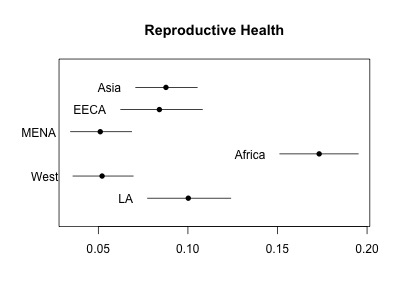
\includegraphics[width=1\linewidth]{2}
  \label{fig:sfig1}
\end{subfigure}%
\begin{subfigure}{.5\textwidth}
  \centering
  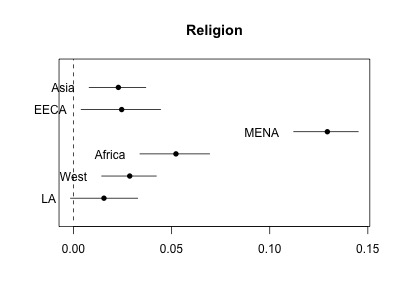
\includegraphics[width=1\linewidth]{3}
  \label{fig:sfig2}
\end{subfigure}
\begin{subfigure}{.5\textwidth}
  \centering
  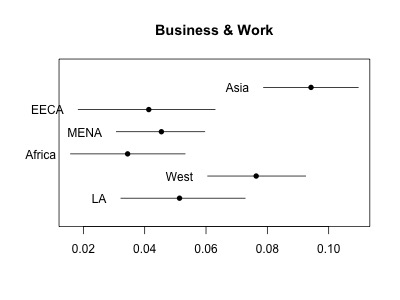
\includegraphics[width=1\linewidth]{4}
  \label{fig:sfig2}
\end{subfigure}
\begin{subfigure}{.5\textwidth}
  \centering
  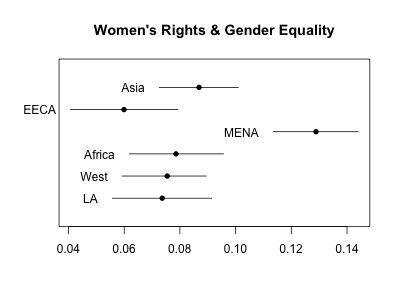
\includegraphics[width=1\linewidth]{12}
  \label{fig:sfig2}
\end{subfigure}
\caption{Expected Document Proportions of 4 Topics}
\label{fig:fig}
\end{figure}

\subsection{Modeling Hypothesis 2}

The reader may find these results unsurprising, given the varying situation of women's rights around the world. In other words, American coverage about women's rights focus more on MENA and Muslim-majority countries, because those are the societies that exhibit the worse sexism. Hypothesis 2 of the gendered orientalist argument, however, argues there is a bias, even when account for realities on the ground.

The dependent variable in Hypothesis 2 is the percentage of coverage devoted to women's rights for a particular country-year (\emph{Rights Focus}). We expect this percentage to be higher for Muslim and Middle Eastern countries than others, even when controlling for women's material status observed in these observations. I operationalized the outcome variable by taking the average proportion of articles assigned to the topic ``Women's Rights \& Gender Equality," weighted by number of words in each article. In other words, I sum the number of words about ``Women's Rights \& Gender Equality" and divide it by the total number of words across all articles in that country-year.  This gives us an estimate of the degree to which the American media focused on this topic relative to others for each observation, ranging from 0 to 1.

The dependent variable \emph{Rights Focus} is then regressed onto two main explanatory variables in order to test the hypotheses described above. The first is \emph{Women's Rights}, or the material status of women's rights, using the same indicator in the first hypothesis. The second is whether the observation represents a Muslim or Middle Eastern country, again using the same indicators as above: the continuous \emph{Percentage Muslim} ranging from 0 to 1, the dichotomous \emph{Muslim Majority}, and the dichotomous \emph{MENA} variables. 

I also include two controls that may affect the rights language in reporting. First, coverage of women's rights may be driven by the general state of human rights protections in certain countries. For instance, the poorer a country?s rights protections, the more coverage it may receive on its rights situation in general, including women?s rights. For this reason, I include a \emph{Democracy} variable, as described above. Alternatively, if a country exhibits a severe level of human rights violations, women?s rights and gender equality might take a backseat to other issues, such as ``Gender Based Violence" or ``Combat." To account for the impact of general human rights abuses, I include a \emph{Physical Integrity Rights} variable, also from the CIRI dataset \footnote{The variable is composed of the four integrity rights variables, including disappearance, extra-judicial killing, political imprisonment, and torture. It is a nine-point scale that ranges from a minimum of zero to a maximum of eight, where zero indicates no respect for physical integrity rights and eight indicates full respect for those rights (Cingranelli and Richards 2012). The data is available to 2011. It should be noted that there are alternative measures for the state of human rights protections used in the literature, such as the CIRI?s Empowerment Rights Index, and the Political Terror Scale measures. I chose the Physical Integrity Index in the models discussed below, but I also estimated models using these two alternative measures, with the same substantive results.} and \emph{Democracy}. 

I model using a heck 

% Table created by stargazer v.5.1 by Marek Hlavac, Harvard University. E-mail: hlavac at fas.harvard.edu
% Date and time: Thu, Sep 24, 2015 - 17:53:02
\begin{table}[!htbp] \centering 
  \caption{} 
  \label{} 
\begin{tabular}{@{\extracolsep{5pt}}lccc} 
\\[-1.8ex]\hline \\[-1.8ex] 
%\\[-1.8ex] & \multicolumn{3}{c}{\textbf{Proportion of Coverage about Women's Rights}} \\ 
\\[-1.8ex] & \textbf{Model 1} & \textbf{Model 2} & \textbf{Model 3}\\ 
\hline \\[-1.8ex] 
 Intercept & 0.094$^{***}$ & 0.096$^{***}$ & 0.090$^{***}$ \\ 
  & (0.011) & (0.011) & (0.011) \\ 
  Lagged DV & 0.084$^{**}$ & 0.085$^{**}$ & 0.084$^{**}$ \\ 
  & (0.041) & (0.042) & (0.041) \\ 
  Women's Rights Index & $-$0.016$^{***}$ & $-$0.019$^{***}$ & $-$0.015$^{**}$ \\ 
  & (0.006) & (0.006) & (0.006) \\ 
  Muslim Majority & 0.042$^{***}$ &  &  \\ 
  & (0.008) &  &  \\ 
  MENA &  & 0.046$^{***}$ &  \\ 
  &  & (0.009) &  \\ 
  Muslim Percentage &  &  & 0.046$^{***}$ \\ 
  &  &  & (0.009) \\ 
  Democracy & $-$0.0002 & 0.00002 & $-$0.0002 \\ 
  & (0.0005) & (0.0005) & (0.0005) \\ 
  Physican Integrity Rights & 0.002 & 0.002 & 0.002$^{*}$ \\ 
  & (0.001) & (0.001) & (0.001) \\ 
  IMR1 & $-$0.003 & 0.0004 & $-$0.003 \\ 
  & (0.005) & (0.005) & (0.005) \\ 
 N & 1116 & 1116 & 1114 \\ 
R-squared & 0.504 & 0.505 & 0.504 \\ 
Adj. R-squared & 0.501 & 0.502 & 0.501 \\ 
Residual Std. Error & 0.091  & 0.091  & 0.091\\ 
 & (df = 1109) & (df = 1109) &  (df = 1107)  \\
F Statistic & 161.037$^{***}$ & 161.564$^{***}$  & 160.791$^{***}$  \\ 
  & (df = 7; 1109) & (df = 7; 1109) & (df = 7; 1107) \\ 

\hline \\[-1.8ex] 
\multicolumn{4}{l}{$^{***}$p $<$ .01; $^{**}$p $<$ .05; $^{*}$p $<$ .1} \\ 
\multicolumn{4}{l}{Robust standard errors clustered on country appear in parentheses.}\\ 
\multicolumn{4}{l}{Selection model equivalent to model summarized in Table \ref{table:logit}} \\ 
\end{tabular} 
\end{table}  

\newpage

\bibliographystyle{apsr}
\bibliography{rights}

\end{document}  